\chapter{Momentum Corrections}
\label{cha:MoCo}
%
The CLAS detector may have some small misalignments and imperfections in the magnetic field that can cause a particle's reconstructed momentum to be slightly off.
This effect can be corrected by studying well known processes, such as elastic events ($ep \rightarrow ep$), Bethe-Heitler events ($ep \rightarrow ep\gamma$), and exclusive events such as $ep \rightarrow e\pi^+n$.
%%%The correction functions used for this analysis were developed by Marco Mirazita \cite{MirazitaMoCo}.
A set of correction functions were determined in order to shift the kinematics of these events to their proper values \cite{MirazitaMoCo}.
The following section show results with and without the corrections to demonstrate their efficacy.
%
\section{Electron Momentum Corrections}
\label{sec:eMoCo}
%
A first step in checking the efficacy of electron momentum corrections is to look at the missing mass distribution of $ep \rightarrow eX$ events near the proton mass, which are elastic events (missing mass is the same as $W$ in this context).
As seen in figures~\ref{fig:W_eX_without} and~\ref{fig:W_eX_with}, the momentum corrections produce an improvement in the mean value (bringing it closer to the proton mass) and in the width (making it narrower) of the elastic peak.
When $W$ is plotted as a function of $\phi_{e-}^{lab}$, a visible improvement in the symmetry of the distribution is present (see figures~\ref{fig:WVphi_eX_without} and~\ref{fig:WVphi_eX_with}).
%
\begin{sidewaysfigure}[htp]
\centering
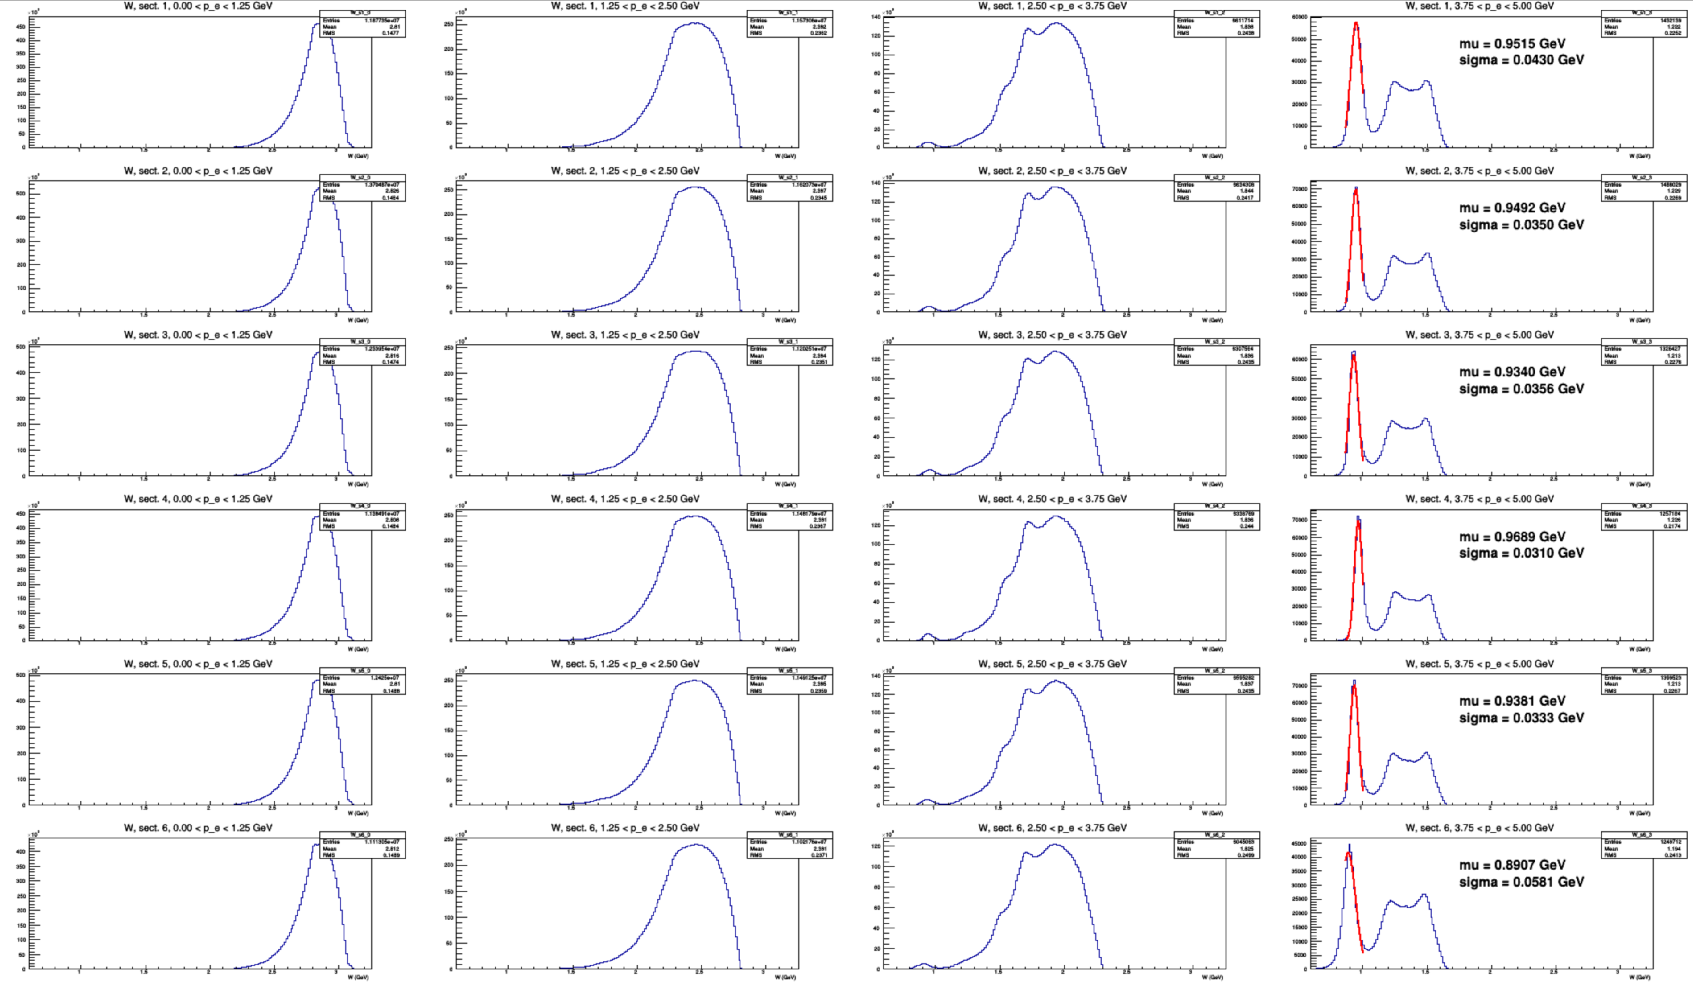
\includegraphics[width=8.5in]{figures/W_eX_without.png}
\caption{Plots of $W$ for $ep \rightarrow eX$ events without momentum corrections. The top row is sector 1, the second row is sector 2, etc. The columns are bins of electron momentum (4 bins from 0 - 5 GeV). The elastic peak becomes visible at higher momenta and is fit with a Gaussian.}
\label{fig:W_eX_without}
\end{sidewaysfigure}
%
\begin{sidewaysfigure}[htp]
\centering
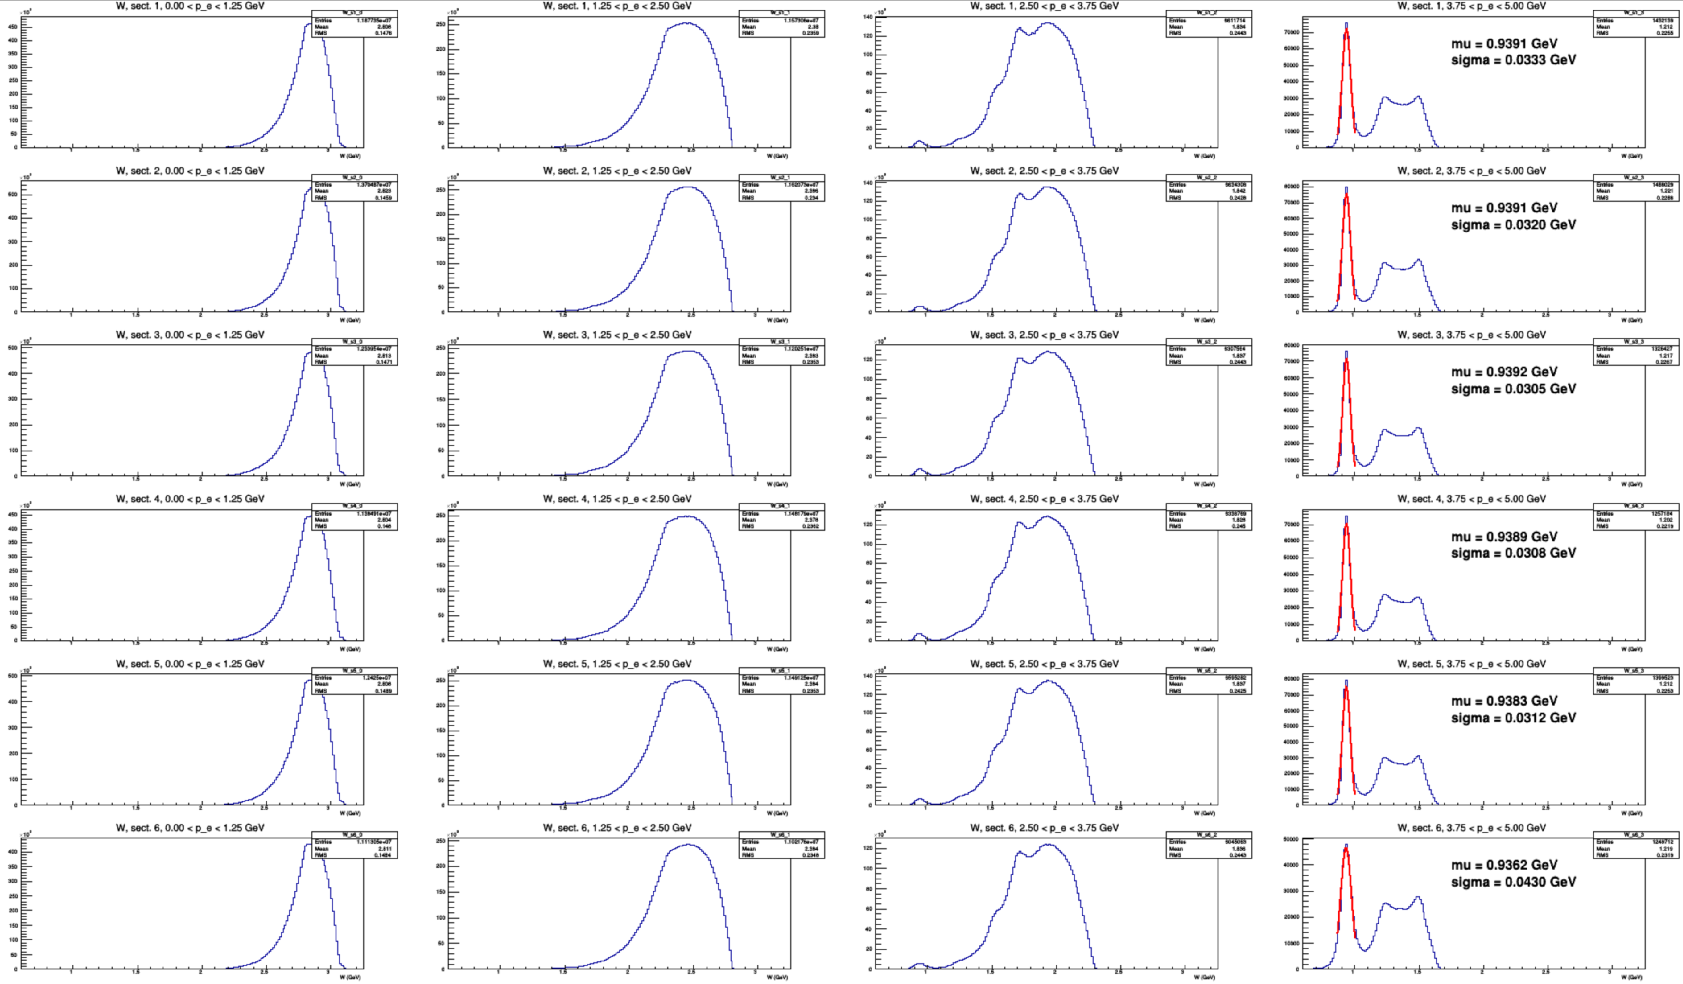
\includegraphics[width=8.5in]{figures/W_eX_with.png}
\caption{The same plots as in figure~\ref{fig:W_eX_without} but with momentum corrections. The mean value (mu) and width (sigma) are both improved for each sector.}
\label{fig:W_eX_with}
\end{sidewaysfigure}
%
\begin{sidewaysfigure}[htp]
\centering
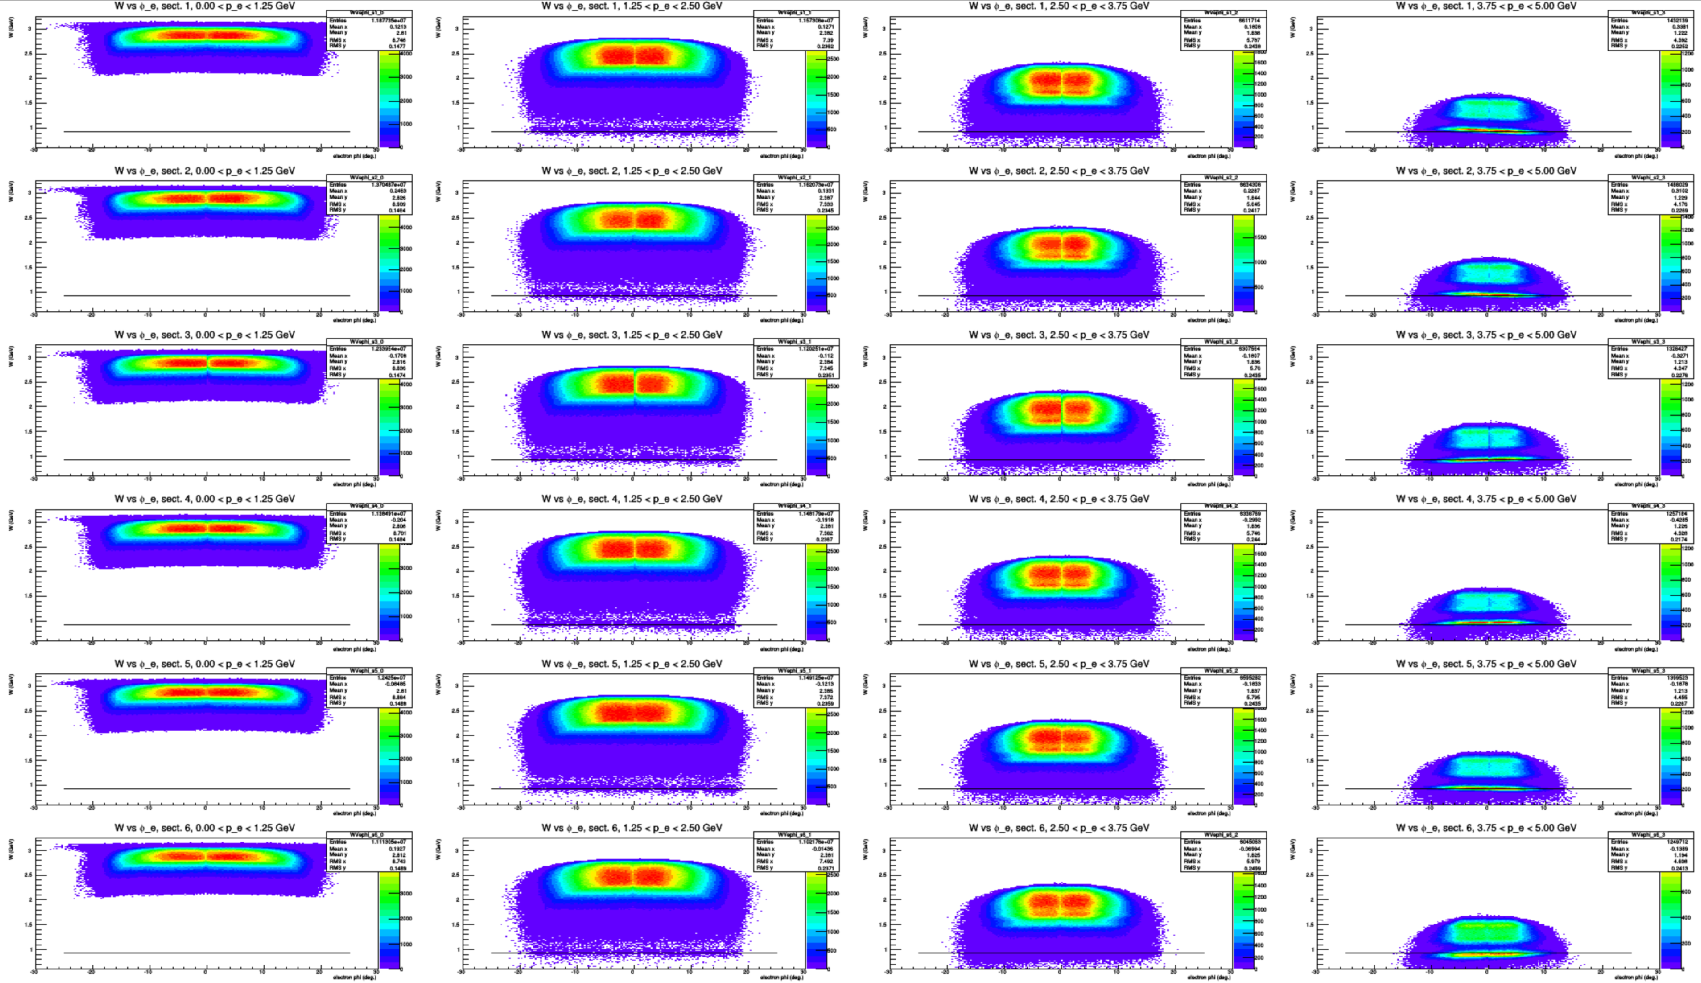
\includegraphics[width=8.5in]{figures/WVphi_eX_without.png}
\caption{Plots of $W$ vs $\phi_{e-}^{lab}$ (relative to the center of the sector) for $ep \rightarrow eX$ events without momentum corrections. The top row is sector 1, the second row is sector 2, etc. The columns are bins of electron momentum (4 bins from 0 - 5 GeV). The elastic peak becomes visible at higher momenta, the black horizontal line shows the location of the proton mass.}
\label{fig:WVphi_eX_without}
\end{sidewaysfigure}
%
\begin{sidewaysfigure}[htp]
\centering
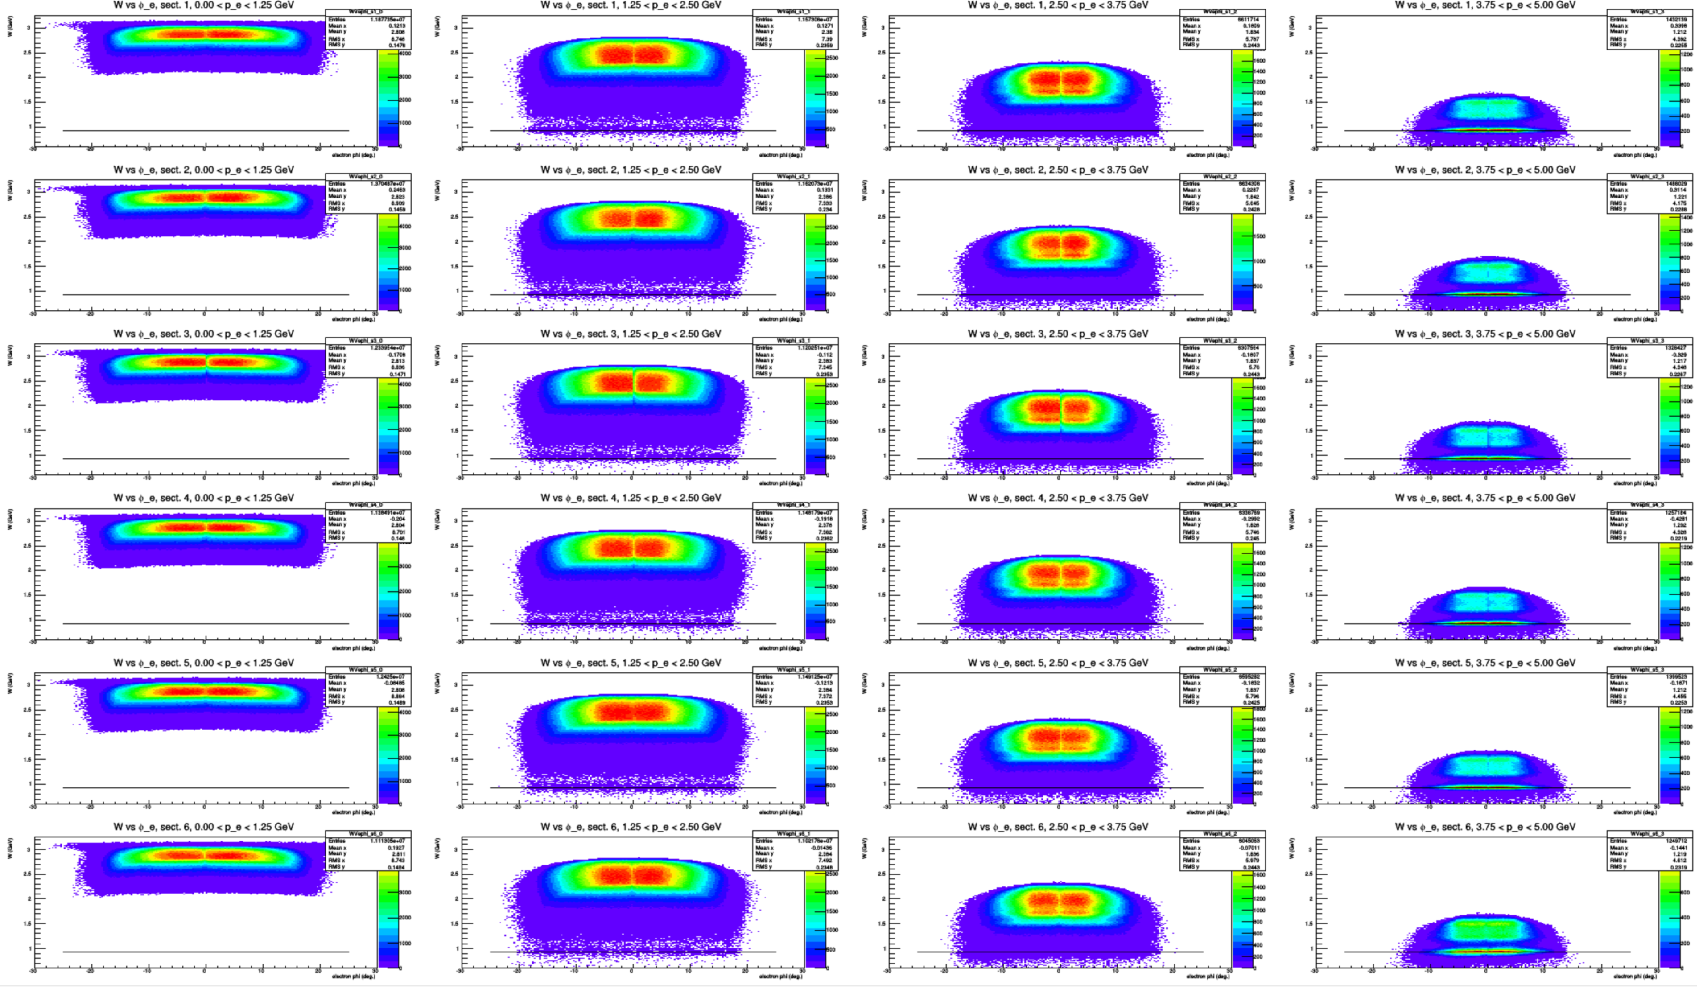
\includegraphics[width=8.5in]{figures/WVphi_eX_with.png}
\caption{The same plots as in figure~\ref{fig:WVphi_eX_without} but with momentum corrections. The symmetry of the distribution is improved for each sector.}
\label{fig:WVphi_eX_with}
\end{sidewaysfigure}

Although the momentum corrections produce an improvement in the $W$ distributions of elastic events, the overlap in phase space coverage between elastic events and SIDIS events is small.
In order to have greater confidence in the momentum corrections, a process with a phase space coverage similar to that of SIDIS events must be studied.
This is done using Bethe-Heitler events.
Bethe-Heitler events are selected using the following criteria: an electron and a proton must be reconstructed, the missing mass squared must be near zero (the photon mass), and the direction of X must be close to either the incoming or outgoing electron direction (since the radiated photon tends to travel in a direction close to that of the electron which radiated it, as shown in figure~\ref{fig:BetheHeitlerDiagrams}).
Since we are looking for events with a phase space coverage similar to that of SIDIS, the additional requirement $W > 2 GeV$ is also added.
%
\begin{figure}[htp]
\centering
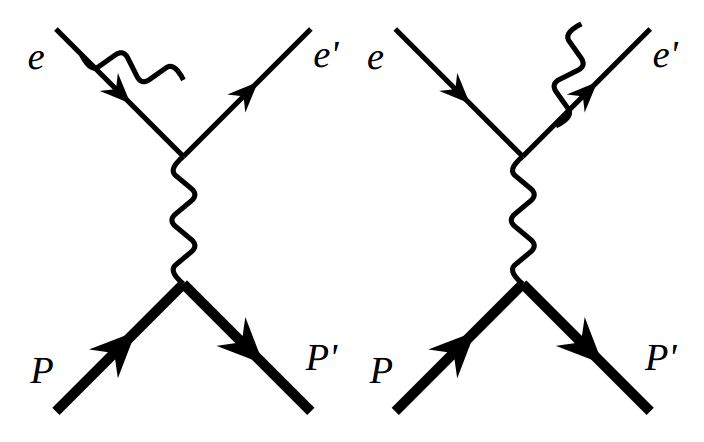
\includegraphics[width=3in]{figures/BetheHeitlerDiagrams.png}
\caption{Left: Pre-radiated Bethe-Heitler process. Right: Post-radiative Bethe-Heitler process. The radiated photon tends to travel in a direction close to that of the electron which radiated it.}
\label{fig:BetheHeitlerDiagrams}
\end{figure}
%

Figure~\ref{fig:h_MX2_eprotX_Wgt2} shows the missing mass squared distribution for $ep \rightarrow epX$ events with $W > 2 GeV$; a cut $-0.05 < M_X^2 < 0.05 GeV^2$ is applied to this quantity to select Bethe-Heitler events.
Furthermore, figure~\ref{fig:eXangles_eprotX_Wgt2} shows the angle between X and the incoming electron ($\Delta\theta_{incoming}$) (left) and the angle between X and the outgoing electron ($\Delta\theta_{outgoing}$) (right) for Bethe-Heitler candidate events.
Events with $\Delta\theta_{incoming} < 0.5$ degrees or $\Delta\theta_{outgoing} < 2$ degrees are kept.
%
\begin{figure}[htp]
\centering
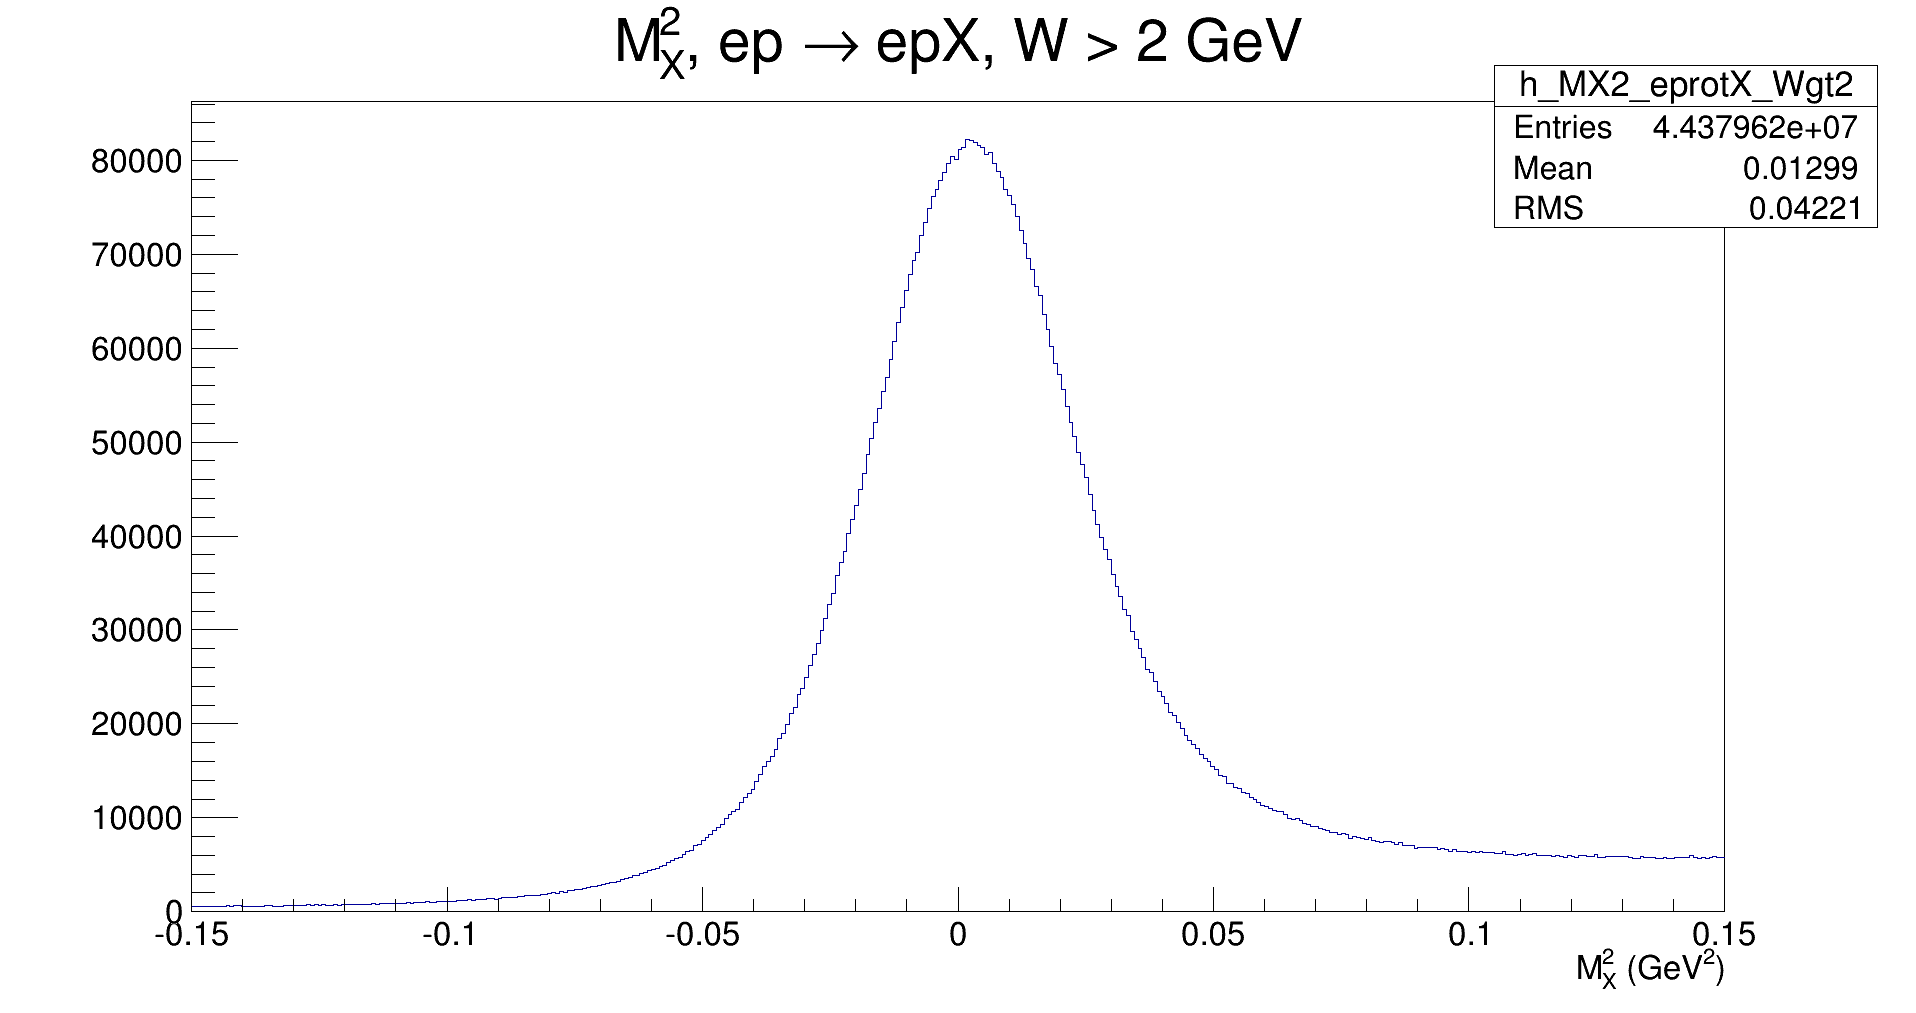
\includegraphics[width=5in]{figures/h_MX2_eprotX_Wgt2.png}
\caption{The missing mass squared distribution for $ep \rightarrow epX$ events with $W > 2 GeV$.}
\label{fig:h_MX2_eprotX_Wgt2}
\end{figure}
%
\begin{figure}[htp]
\centering
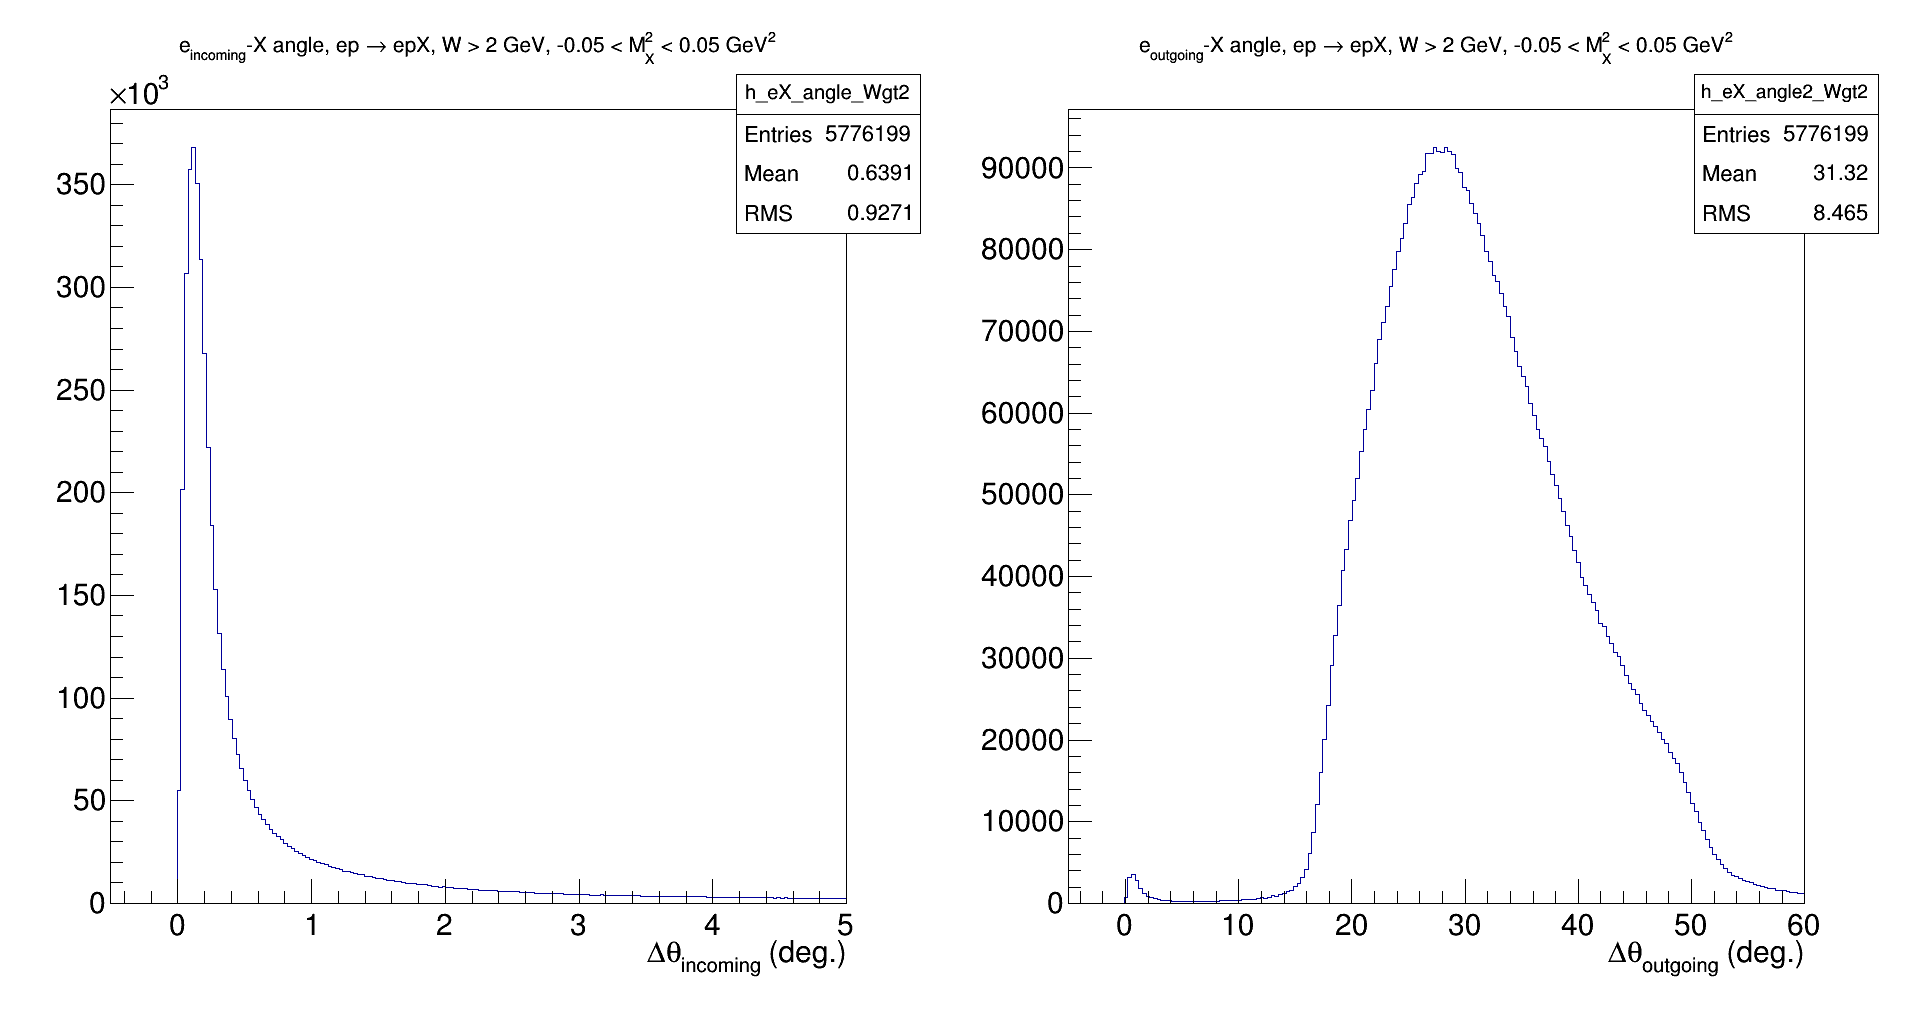
\includegraphics[width=5in]{figures/eXangles_eprotX_Wgt2.png}
\caption{Left: $\Delta\theta_{incoming}$ and right: $\Delta\theta_{outgoing}$ for $ep \rightarrow epX$ events with $W > 2 GeV$ and $-0.05 < M_X^2 < 0.05 GeV^2$.}
\label{fig:eXangles_eprotX_Wgt2}
\end{figure}
%

Returning to the missing mass squared distribution after applying the $\Delta\theta_{incoming}$ and $\Delta\theta_{outgoing}$ cuts (figure~\ref{fig:MX2_BHevents}), it can be seen that the momentum corrections produce a small improvement in the peak position (bringing it closer to zero) while the width does not change significantly.
Likewise, when the missing mass squared is plotted as a function of $\phi_{e-}^{lab}$ (relative to the center of the sector), a visible improvement is noticeable in the symmetry of the distributions after momentum corrections are applied (see figure~\ref{fig:MX2Vphi_BHevents}).
%
\begin{sidewaysfigure}[htp]
\centering
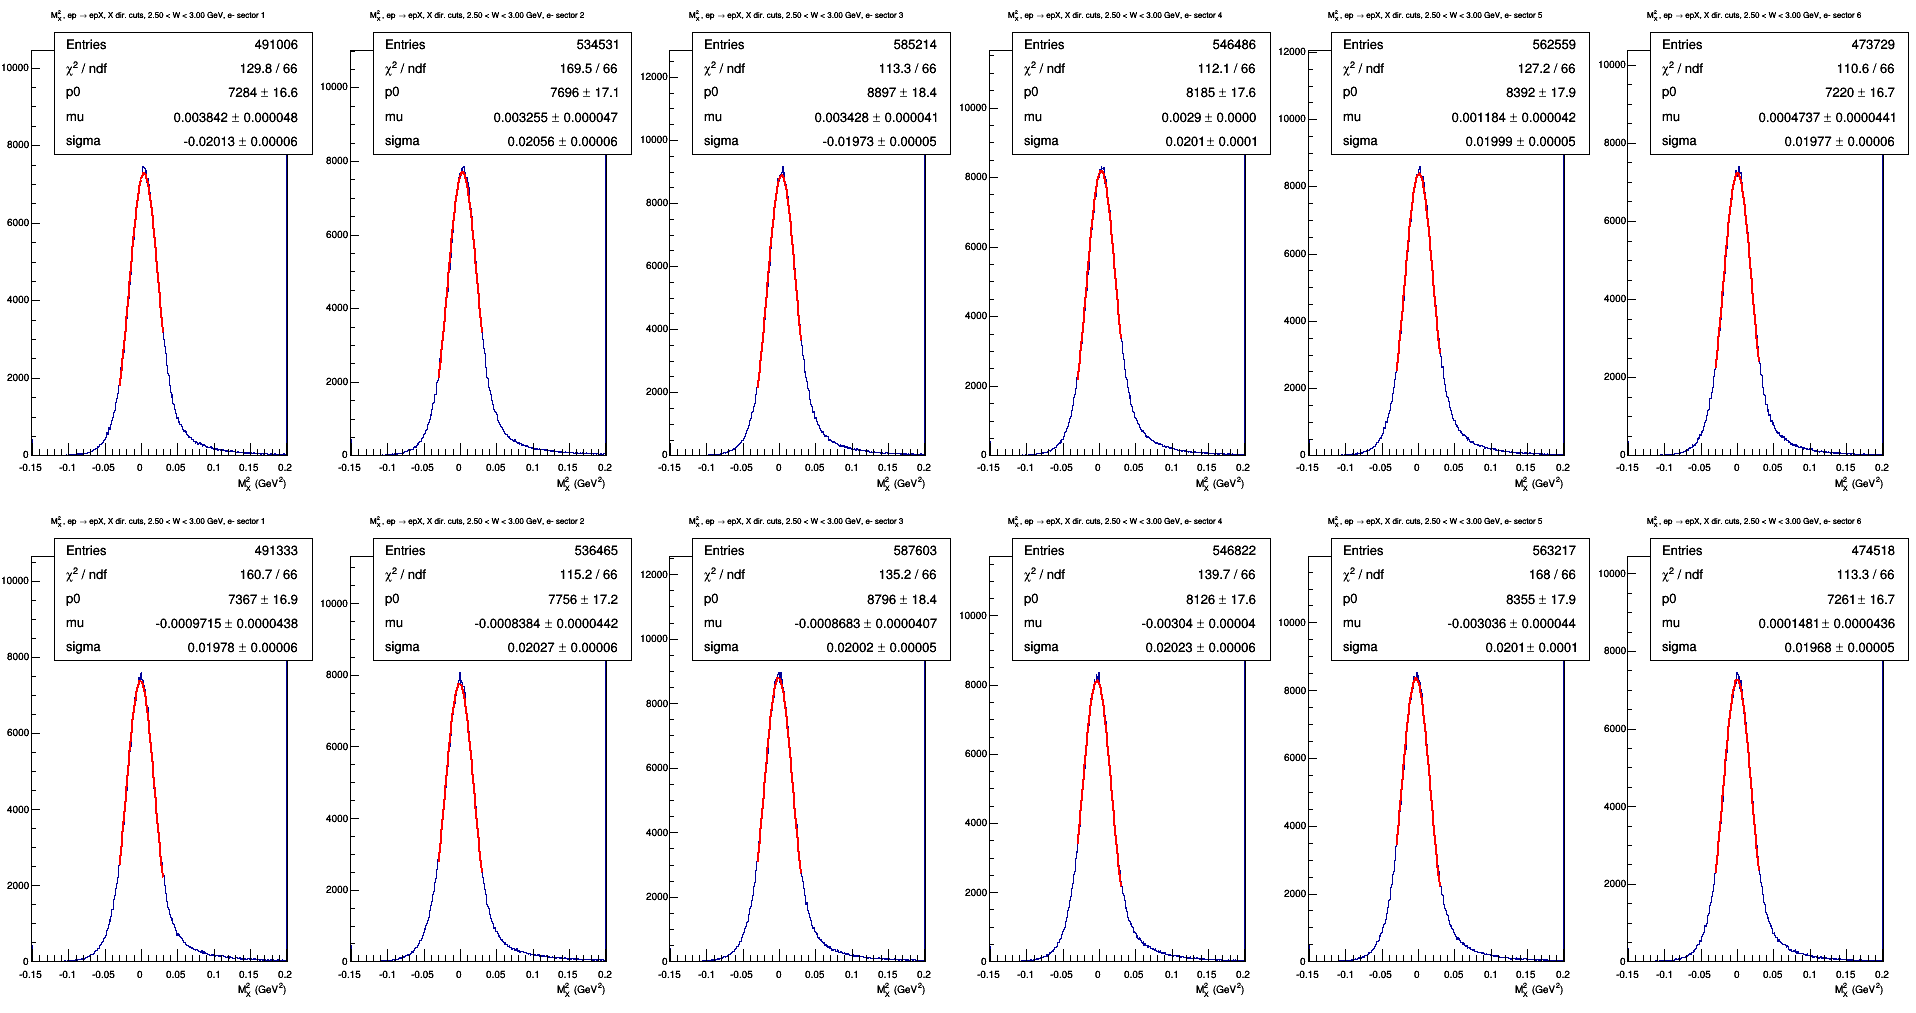
\includegraphics[width=8.5in]{figures/MX2_BHevents.png}
\caption{The missing mass squared distribution for Bethe-Heitler events. The first column is for events with the electron in sector 1, second column sector 2, etc. The top row is without momentum corrections and the bottom row is with the corrections.}
\label{fig:MX2_BHevents}
\end{sidewaysfigure}
%
\begin{sidewaysfigure}[htp]
\centering
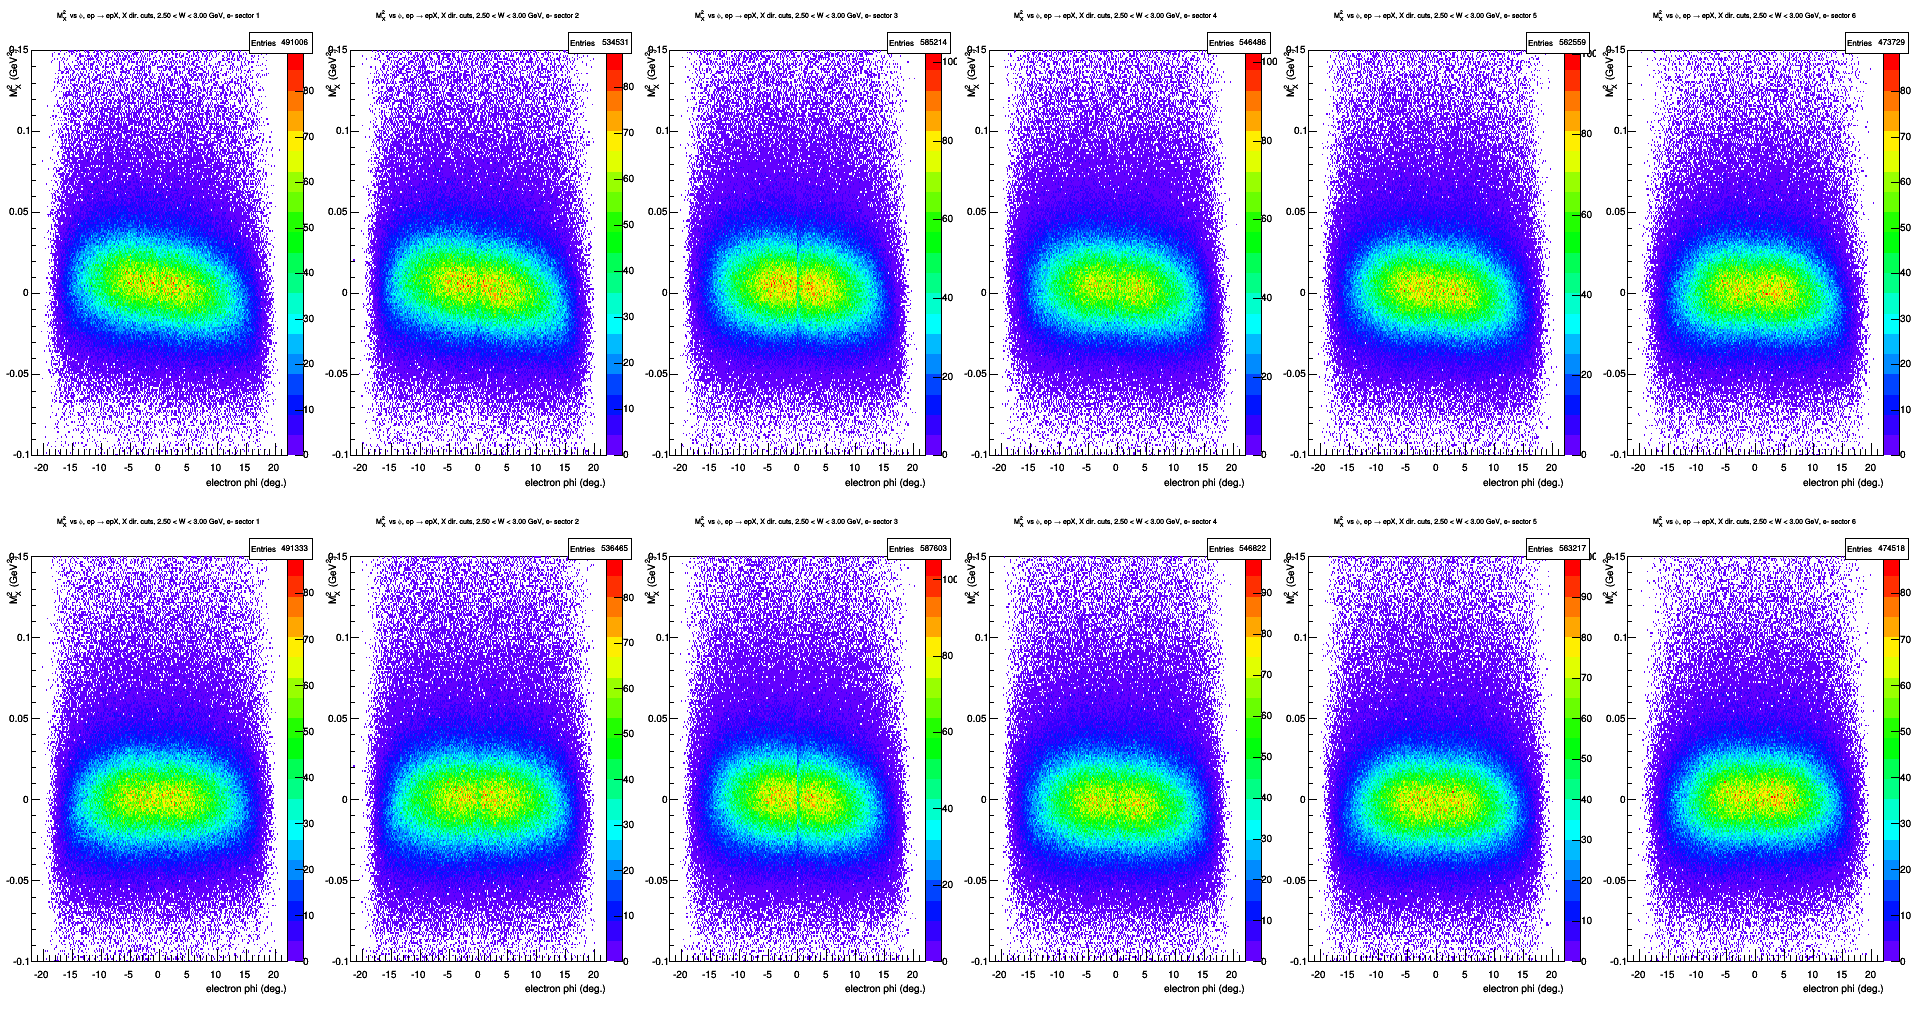
\includegraphics[width=8.5in]{figures/MX2Vphi_BHevents.png}
\caption{The missing mass squared vs $\phi_{e-}^{lab}$ (relative to the center of the sector) distribution for Bethe-Heitler events. The first column is for events with the electron in sector 1, second column sector 2, etc. The top row is without momentum corrections and the bottom row is with the corrections.}
\label{fig:MX2Vphi_BHevents}
\end{sidewaysfigure}
%

The $Q^2-x$ space for Bethe-Heitler events with $W > 2 GeV$ is plotted in figure~\ref{fig:QQVx_BHevents} to confirm that the phase space coverage of these events is similar to that of SIDIS events.
%
\begin{figure}[htp]
\centering
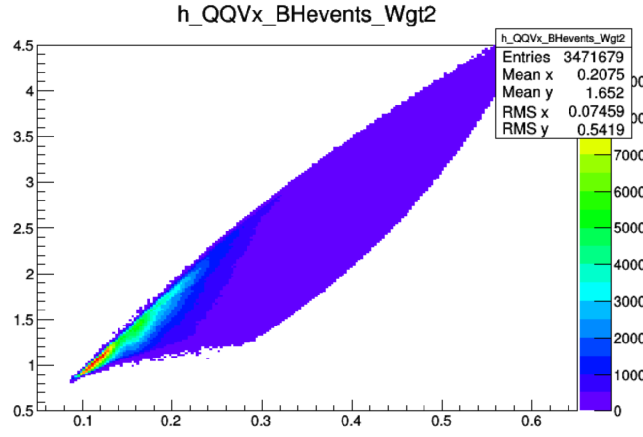
\includegraphics[width=5in]{figures/QQVx_BHevents.png}
\caption{The $Q^2-x$ space for Bethe-Heitler events with $W > 2 GeV$. This coverage is similar to that of SIDIS events which makes Bethe-Heitler events useful for studying momentum corrections in a SIDIS analysis such as this one.}
\label{fig:QQVx_BHevents}
\end{figure}
%

The electron momentum correction functions studied here have been shown to improve the kinematic distributions of well know processes with similar phase space coverage as SIDIS events, making them suitable for this analysis.

\clearpage % should prevent a backlog of figures from piling up
